%% 
%% Copyright 2019-2020 Elsevier Ltd
%% 
%% This file is part of the 'CAS Bundle'.
%% --------------------------------------
%% 
%% It may be distributed under the conditions of the LaTeX Project Public
%% License, either version 1.2 of this license or (at your option) any
%% later version.  The latest version of this license is in
%%    http://www.latex-project.org/lppl.txt
%% and version 1.2 or later is part of all distributions of LaTeX
%% version 1999/12/01 or later.
%% 
%% The list of all files belonging to the 'CAS Bundle' is
%% given in the file `manifest.txt'.
%% 
%% Template article for cas-dc documentclass for 
%% double column output.

%\documentclass[a4paper,fleqn,longmktitle]{cas-dc}
\documentclass[a4paper,fleqn]{cas-dc}

%\usepackage[authoryear,longnamesfirst]{natbib}
%\usepackage[authoryear]{natbib}
\usepackage[numbers]{natbib}

\usepackage[font=footnotesize, justification = centering]{caption}
\usepackage[font=footnotesize]{subcaption}
\usepackage{amsmath}
\usepackage[ruled,linesnumbered]{algorithm2e} %for writing pseudocodes
\usepackage{graphicx}
\usepackage{float}

%%%Author definitions
\def\tsc#1{\csdef{#1}{\textsc{\lowercase{#1}}\xspace}}
\tsc{WGM}
\tsc{QE}
\tsc{EP}
\tsc{PMS}
\tsc{BEC}
\tsc{DE}
%%%

\begin{document}
\sloppy	

\let\WriteBookmarks\relax
\def\floatpagepagefraction{1}
\def\textpagefraction{.001}
\shorttitle{Versatility in Controller Placement Approaches through Graph Theory and Greedy Search Techniques}
\shortauthors{TI Aziz et~al.}

\title [mode = title]{Versatility in Controller Placement Approaches through Graph Theory and Greedy Search Techniques}

%\tnotetext[1]{This document is the results of the research
%   project funded by the National Science Foundation.}

%\tnotetext[2]{The second title footnote which is a longer text matter
%   to fill through the whole text width and overflow into
%   another line in the footnotes area of the first page.}



\author[1]{Talha Ibn Aziz}[type=editor,
                        auid=000,bioid=1,
                        role=Researcher,
                        orcid=0000-0001-8747-8119]
\cormark[1]
\ead{taziz@ualberta.ca}
\ead[url]{sites.google.com/view/talha-ibn-aziz}

%\credit{Conceptualization of this study, Methodology, Software}

\address[1]{Department of Computing Science, University of Alberta}

\author[2]{Muhammad Mahbub Alam}[%
   role=Supervisor,
   ]
\ead{mma@iut-dhaka.edu}
%\ead[URL]{www.sayahna.org}

%\credit{Data curation, Writing - Original draft preparation}

\author[2]{Md Sakhawat Hossen}[role=Co-ordinator,]
\ead{sakhawat@iut-dhaka.edu}

\address[2]{Department of Computer Science and Engineering, Islamic University of Technology}

\cortext[cor1]{Corresponding author}
%\fntext[fn1]{This is the first author footnote. but is common to third
%  author as well.}
%\fntext[fn2]{Another author footnote, this is a very long footnote and
%  it should be a really long footnote. But this footnote is not yet
%  sufficiently long enough to make two lines of footnote text.}

%\nonumnote{This note has no numbers. In this work we demonstrate $a_b$
%  the formation Y\_1 of a new type of polariton on the interface
%  between a cuprous oxide slab and a polystyrene micro-sphere placed
%  on the slab.
%  }

\begin{abstract}
Software Defined-Networks (SDNs) decouple the traditional protocol stack into the control plane and the data plane consisting of - controllers and switches, respectively. The controllers are placed in the network considering numerous fundamental parameters like flow-setup latency, switch-controller control traffic, route synchronization latency, reliability, and security. While many researchers address the resultant Controller Placement Problem (CPP), very few provide a thorough and efficient process that considers multiple core parameters. In this paper, we propose three algorithms to cluster the network, place controllers, and assign switches dynamically to controllers in polynomial time. Extensive simulations on two hundred and forty-three (243) existing network topologies suggest that our approach outperforms current state-of-the-art controller placement algorithms in terms of flow-setup latency and traffic-awareness.
\end{abstract}

\begin{keywords}
SDN \sep CPP \sep controllers \sep flow-setup \sep latency \sep control traffic
\end{keywords}


\maketitle

\section{Introduction}
\noindent The booming usage growth of the Internet, and the integration of a plethora of Internet of Things (IoT) devices into the network system - causes a shortage of network management resources. The complexity of configuring the already-troublesome network, is further increased by the amalgamation of switches from various vendors. In light of the above-mentioned predicament, a novel network architecture known as Software Defined Network (SDN) is proposed, which has been a center-stage of cutting-edge research for the past few decades. SDNs distribute the traditional network-layer functions to simplify network management and configuration, making efficient use of scarce resources. The forwarding capabilities are retained by the switches and routers, while new agents are introduced as the decision making entities. These authoritative devices - namely \textit{controllers}, have superior processing power and memory compared to the switches, which are simplified in terms of both costs and design.

The original SDN architecture \cite{greene2009tr10} includes a single controller, resulting in the formation of bottle-necks, single point of failure, and scalability issues \cite{scalability2013dixit, scalability2013yeganeh}. Consequently, the multiple-controller architecture is proposed for larger networks; however, the solution comes with its own NP-Hard Controller Placement Problem (CPP). The CPP deals with placing an optimal number of controllers to optimize one or more constraints - network latencies, deployment costs, energy consumption, reliability, and resilience \cite{zhang2017survey, singh2018survey, cox2017survey}. In this paper, we propose a novel controller assignment method which minimizes the following:

	\textbf{(1) Latency:} We minimize two latencies simultaneously, namely, \textit{route synchronization latency} and \textit{flow-setup latency}. When there is a change in the network, the concerned controllers and switches are notified immediately. The delay produced here is called the route-synchronization latency. When a new flow arrives at a switch, the flow-setup process is initiated, through which the corresponding controller calculates a new path and notifies the concerned switches. The total delay incurred in this process is called the flow-setup latency.
	
	\textbf{(2) Controller response time and Load imbalance:} Due to the influx of numerous new flows, several query packets from multiple switches impose on the controllers. The great volume of processing required by a controller to facilitate the smooth operation of the network is called the \textit{load of a controller}. Imbalanced distribution of load can lead to an exponential increase in controller response times.
	
The processing delay of SDN switches is significantly reduced compared to traditional networks and propagation latencies are negligible due to greater wave propagation velocities. Therefore, the overall flow-setup latency relies primarily on transmission latency and queuing latency of control packets \cite{forouzan2006data}. Our proposed method aims to divide the network into \textit{k} balanced clusters and place a controller in each cluster to reduce transmission latency. Furthermore, the controller response time is improved through dynamic load balancing, which reduces queuing latency. 

Most research perform optimization of a specific latency or parameter instead of providing a complete system, while a few of them address multiple parameters simultaneously \cite{lange2015multi, sallahi2015optimal}. However, they either provide exhaustive solutions or reduce accuracy to improve efficiency in terms of time and/or space complexity. To the best of our knowledge, there is no such method that clusters the network, place controllers considering both inter-controller and intra-controller latency, and assigns switches dynamically to minimize flow setup latency, route synchronization latency, load imbalance, and controller response times in polynomial complexity. Therefore, we develop multiple algorithms to address the problem at hand, and our main contributions are summarized as follows:
\begin{itemize}
	\item We minimize overall flow-setup latency and route synchronization latency while placing controllers. Furthermore, we provide a way to trade-off between inter-controller and intra-controller latencies for network managers.
	
	\item We develop three polynomial-time algorithms to cluster the network, place controllers and balance controller loads. We also suggest an optimal number of controllers.
	
	\item Our proposed method is traffic-aware and reduces controller response time by balancing controller loads in real-time. It can be improved further to work with any network parameter.
	
	\item We perform simulations on 243 existing network topologies and our simulations show that our method outperforms state-of-the-art algorithms for controller placement in terms of flow-setup latency, controller response time, and load balancing.
\end{itemize}


The remainder of our paper consists of the background and related works in Section \ref{background}, the problem formulation in Section \ref{sysMod}, the detailed proposed mechanism in Section \ref{proposal}, the performance analysis in Section \ref{simulations}, the simulation results in Section \ref{simulationResults}, and the conclusion in Section \ref{conclusion}.

\section{Background and Related Works} \label{background}
\noindent Several research papers have addressed multiple aspects of the Controller Placement Problem (CPP) in the last decade. Heller et al. \cite{heller2012latency} study the effects of different latencies on overall network throughput through exhaustive controller deployment and generate two essential questions - \textit{How many controllers are needed?} and \textit{Where in the topology should they go?} Solutions to the CPP address these questions by optimizing various parameters when placing controllers, namely - switch-controller and controller-controller delays, route synchronization latency, flow-setup latency, reliability and resilience, deployment costs, traffic-awareness, etc. Some of the notable works are mentioned in this section along with the parameters they addressed.

Li et al. \cite{li2020latency} minimize the average switch-controller transmission delay to achieve effective deployment of multiple controllers in a continuous two-dimensional space by adopting the PSO (particle swarm optimization). Das et al. \cite{das2020latency} presents a Steiner tree-based model that analyses the network state synchronization delay between the controllers by minimizing inter-controller latency. The model addresses both failure-free and post-failure scenarios to make the placement resilient. Multiple researchers explicitly address the reliability and resilience of multiple controller placement. Hu et al. \cite{hu2013reliability} introduces a metric - expected percentage of control path loss and formulates the reliability-aware control placement problem. Zhang et al. \cite{zhang2011resilience} propose a min-cut based graph partitioning algorithm to place controllers, which aims at maximizing the resilience of the network and shows its advantage over greedy algorithms. Ashrafi et al. \cite{ashrafi2020reliability} address this issue by developing a mathematical model to minimize latency while taking all failure scenarios and scalability into consideration. Fan et al. \cite{fan2020reliability} minimize the average drop-rate of flow set-up requests due to single-link failure using two algorithms - Reliability Aware Controller Placement (RAC) and Fast-RAC (FRAC). Yang et al. \cite{yang2020security} introduce a greedy heuristic algorithm for single-link failures and the Monte Carlo Simulation for multi-link failures

Placing minimal controllers makes the SDN vulnerable to failures and security attacks. Contrarily, deploying maximal controllers reduces delays, response times of the controllers, and throughput of the network; it is, however, not feasible in terms of cost and inefficient in terms of resources. Sallahi et al. \cite{sallahi2015optimal} propose a mathematical model to determine the optimal number of controllers and their locations in a network while minimizing the cost of the SDN. Chaudhary et al. \cite{chaudhary2020cost} develop the Placement Availability Resilient Controller (PARC) scheme to provide a stable partitioning of the network, a co-operative game theory-based localization of controllers, and an optimal controller number calculation including extra backup controllers while minimizing network cost. Several research proposals also address the wireless paradigm of SDN - Dvir et al. \cite{dvir2019wireless} minimize propagation latency, maximize throughput, and link failure probability while placing controllers. Toufga et al. \cite{toufga2020vehicle} propose and Integer Linear Programming (ILP) based placement method which dynamically changes controller placement based on road traffic fluctuations for Software-Defined Vehicular Networks (SDVNs). Papa et al. \cite{papa2020satellite} place controllers in large-scale satellite networks to minimize the average flow setup latency with respect to varying traffic demands.

The fluctuations of switch-controller control traffic impose varying loads on the controllers. Consequently, the performance of a controller is significantly reduced when its load exceeds its processing capacity. Wang et al \cite{wang2011load} distributes the traffic using wildcard rules on supported switches to transfer traffic to OpenFlow \cite{hu2014survey} server replicas. Yao et al. \cite{yao2014capacitated} define the Capacitated Controller Placement Problem (CCPP) which takes loads of controllers into consideration and also introduces an efficient algorithm to solve it. Yao et al. \cite{yao2015controller} propose a multi-controller load balancing approach called HybridFlow for software-defined wireless networks, which is a flow-based dynamic solution. Chen et al. \cite{chen2018load} propose a load balancing scheme that provides quality of service (QoS) for machine-to-machine (M2M) networks through traffic identification and rerouting. Choumas et al. \cite{choumas2020oittraffic} assess and explore control-traffic minimization and devise multiple heuristic algorithms to propose an efficient solution. Coronado et al. \cite{coronado2017wiload} propose - \textit{Wi-Balance}, an algorithm that balances traffic load and maintains an equal division of network resources.
Qilin et al. \cite{qilin2015load} improve traffic scheduling by reducing the number of flow tables. Schutz et al. \cite{schutz2020load} formalizes the CPP mathematically to place controllers while keeping a balanced load distribution.

The explosive amount of data traffic generated due to the advent of the Internet of Things (IoT) and improvement of Mobile networks demands better and more efficient load balancing algorithms. Under these circumstances, multiple variations of stable matching algorithms are proposed to ensure maximum utilization of available resources. Wang et al. in \cite{wang2016load} propose a combination of matching theory and conditional games to perform load balancing of controllers. Filali et al. \cite{filali2018sdn} formulate the CCPP as a one-to-many matching game and use a well-known stable matching algorithm - Multistage Deferred Acceptance Algorithm (MSDA) \cite{fragiadakis2016matching} to solve it.

\section{Problem Formulation and Assumptions} \label{sysMod}
\noindent Systematic segregation of the network layer into control and data planes require the division of larger networks into multiple sub-networks, where each sub-network is governed by a single controller.

%sets of switches eqn and sub-network=> cluster
We represent the network as a weighted bi-directional graph $G=(S,E)$, where $S$ represents the set of switches (or nodes) and $E$ represents the set of links (or edges) between the switches. The weights of the edges represent the transmission delays, which is the reciprocal of the bandwidth of the links. The graph $G$ is clustered into $k$ mutually exclusive and collectively exhaustive sets of switches (i.e., sub-networks) denoted by $S_i$, where $i=1,2,....,k$. Switches in a sub-network forward packets following a set of rules, using \textit{flow-tables}. However, when a new \textit{flow} arrives, the concerned switch sends a query packet to the controller of the sub-network. The controller notifies the switches in the path of the flow about the new rule. It also notifies the respective controllers of the switches in the path (unless the switch is in the same sub-network).

The flow setup procedure for a switch can be divided into three phases, 1) the switch sends a query packet to its controller, 2) after a period of queuing delay (if any), the controller processes the query and takes a routing decision, and finally, 3) the controller informs all the switches of the flow-path about the new rule. The time required to complete all the three phases is called the \textit{flow-setup latency}.

The delay incurred by the first phase of the flow-setup procedure depends on the link between the concerned switch and controller. The delay in the second phase is the time a controller takes to decide a flow-path, and is called the \textit{controller response time}. The response time can be calculated if the \textit{loads} of the switches and the controllers, and the \textit{processing power} of the controllers are known. The total number of query packets generated by a switch in unit time is the load of the switch (hereafter referred to as \textit{switch-load}) and the total number of query packets generated by all the switches in a sub-network is the load of the controller (hereafter referred to as \textit{controller-load}).

We assume that both the arrival times and the service times of the queries follow a Poisson process like \cite{wang2016load}. Therefore, the delays associated with the queries at the controller can be modeled as an M/M/1 queue and the average system time (i.e., the waiting time and service time) can be determined using Little's Law as follows \cite{wang2016load}:

\begin{equation} \label{eqn:cresponse}
RT_{avg} = \frac{1}{(Power_{C_i} - Load_{C_i})}
\end{equation}
where $Power_{C_i}$ and $Load_{C_i}$ of any controller $C_i$ in the network are the maximum processing power and the load of the controller, respectively .

When all the controllers are overloaded and working at full capacity, the system is unstable as the queues will grow unboundedly. Therefore, balancing the network load does not contribute to the performance of the system. However, when overall network load does not exceed the system capacity, balancing controller-loads greatly improve throughput and performance, especially when one or more controllers are overloaded. An efficient load-balancing approach in this case, is to assign loads to controllers according to their processing capacity. In order to maintain the balance and avoid controller overload, loads can be distributed constantly as the network operates (\textit{dynamic traffic-awareness}).

The third phase of the flow-setup procedure depends on the controller-switch latencies between the concerned controllers and their respective switches in the flow-path, and the inter-controller latencies among the involved controllers. Furthermore, the time required for a controller to announce any change within its sub-network, namely the route-synchronization latency, is also determined by the controller-switch latency. Therefore, our goal is to divide the network into clusters while,
\begin{enumerate}
	\item placing controllers to minimize the overall flow-setup and route synchronization latencies, and
	\item dynamically balancing the loads among the controllers to reduce average controller response times.
\end{enumerate}
For simplicity, we assume that the processing delay of all switch-to-controller control packets is negligible. Furthermore, a controller can only be placed on a switch location and all the controllers have identical processing capacity.

%Flow of the problem formulation should be as follows: first paragraph expresses the network as a graph with nodes and edges (what they represent as well). The second part defines how a network will be divided into sub-networks or clusters (may use the notations S_{i=1,2,...,k}). The third part explains in entirity how the flow setup latency needs to be minimized and how the route synchronization and load imbalance plays a role here and how each of these are minimized (without going into our proposed algorithm). Then start with our goals and the two points that we have already mentioned.

\section{Proposed Methodology} \label{proposal}

\noindent In our proposed method, we develop three algorithms - Latency-based Clustering Algorithm (LBCA), Latency-based Controller Selection Algorithm (LCSA), and Greedy Load Balancing Algorithm (GLBA). LBCA clusters the network into a given number of sub-networks ($k$) and LCSA places a controller in each of the sub-networks, resulting in a static controller-switch assignment. GLBA is a dynamic load balancing algorithm that periodically reassigns switches to avoid over-burdening a controller.

\subsection{Latency-based Clustering Algorithm (LBCA)} \label{lbca}

%In short write in two lines about the subsubsections
\noindent The Latency-based Clustering Algorithm (LBCA) clusters the network in two phases: the first phase selects the cluster-centers and the second phase forms the clusters surrounding the cluster-centers.

\subsubsection{Cluster-center selection}

\noindent Before forming a cluster, LBCA determines the footholds from which a cluster will be created, to ensure that the clusters are not concentrated in a certain region. Consequently, LBCA re-clusters the network to avoid forming geographically irregular clusters (varying shapes and sizes). A recent controller placement algorithm DBC \cite{aziz2019degree}, places controllers based on inter-controller and intra-controller distances. DBC further ensures that these footholds, namely \textit{cluster-heads}, are a minimum distance ($T_d$) apart from each other. However, the cluster-heads are randomly selected and the $T_d$ distance is calculated virtually. Contrarily, LBCA determines the foundations of the clusters based on their average distance from all other nodes. Accordingly, we name the foundations as \textit{cluster-centers} and propose a novel clustering algorithm LBCA.

In a single-controller network, placing the controller at the center - minimizes the controller-switch delay. Considering the network as a graph $G$, the center is the node with the minimum - average or maximum delay - from every other node in $G$ \cite{wilson1979introduction}. The average delay can be calculated as:

\begin{equation} \label{eqn:avgDis}
center_{avg} = \min_{s\in S}\bigg(\frac{\sum_{d\in S, d\ne s}T(s,d)}{|S|-1}\bigg)
\end{equation}

where, $center_{avg}$ is the node with the minimum average delay and $T(s,d)$ is the shortest path distance from node $s$ to $d$.

\begin{equation} \label{eqn:maxDis}
center_{dia} = \min_{s\in S}\bigg(max_{d\in S}\big(T(s,d)\big)\bigg)
\end{equation}

Here, node $center_{dia}$ has the minimum of all the maximum delays in the network and is always on the network diameter.

\begin{figure}
	\centering
	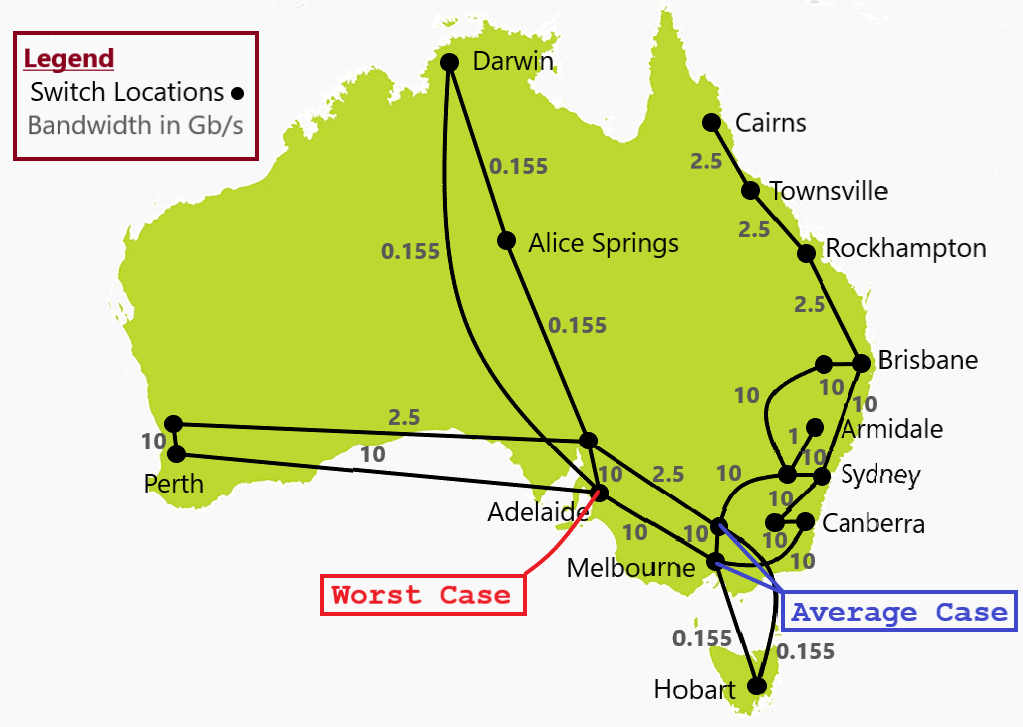
\includegraphics[width=0.9\linewidth]{Images/Aarnet.png}
	\caption{Existing network of Australia (AARNET \cite{knight2011internet}) showing the centers of the network.}
	\label{fig:aarnetcc}
\end{figure}

When the center of the network is determined by the maximum delay or worst-case latency (Equation \ref{eqn:maxDis}), the position of the center can vary greatly in the presence of distant and isolated nodes (Figure \ref{fig:aarnetcc}). Conversely, the average case latency (Equation \ref{eqn:avgDis}) is less affected by outliers or distant nodes. Therefore, we select the node with the minimum average distance ($center_{avg}$) as the center of the network. This solution of the single-controller placement sub-problem, can be extended to place controllers in the multi-controller environment of a larger network, where each controller is placed in a sub-network. To ensure equal division of the network into sub-networks or clusters, the cluster-centers are expected to be equidistant from each other and the clusters must expand from the cluster-centers. This selection of centers in a network is a classical NP-hard problem - \textit{The vertex k-center problem} \cite{kariv1979algorithmic}, which has many sub-optimal approximations. The prosposed algorithm LBCA (Algorithm \ref{algo:lbca}) utilizes the latency among switches to divide the network optimally while ensuring minimum overlapping among neighboring clusters.

\begin{algorithm}
	\SetAlgoLined
	\KwResult{Set of Clusters, $S_i$ }
	$S :=$ set of nodes in network $G$\;
	Calculate shortest path delay $T(a,b)$ between all possible pair of nodes $a$ and $b$ \;
	
	for any $s\in S$, $\overline{T}_s := \frac{\sum_{\forall d\in S} T(s,d)}{|S|-1}$, where $d \ne s$\;
	
	$CC := \varnothing$, $k :=$ required number of controllers\;
	
	\While{$|CC| < k$}{
		Find $s_{cc}$ such that $\overline{T_{s_{cc}}} \le \overline{T_{\forall t\in S}}$\;
		
		$CC := CC \cup \{s_{cc}\}$\;
		
		Create a new cluster $S_i$ which consists of $s_{cc}$ and $\big(\frac{|S|}{k}-1\big)$ nearest neighbors of $s_{cc}$ in terms of hop distance\;
		
		\ForEach{switch $s_i \in S_i$}{
			Subtract $\frac{T(s_i, s)}{|S|-1}$ from $\overline{T_s}$ for all ${s \in S \setminus S_i}$
		}
		$S = S \setminus S_i$
	}
	Discard previous clustering and form new clusters $S_i$ each containing one cluster-center $CC_i$ and all its nearest nodes, where $i=1,2,..,k$\;
	
	\caption{Latency-based Clustering Algorithm (LBCA)} \label{algo:lbca}
\end{algorithm}

%Make the pseudocode simpler and change the paragraph below accordingly
Initially, LBCA calculates the delays between every possible pairs of nodes in terms of shortest source to destination path delays (Algorithm \ref{algo:lbca} Line 2) using Dijkstra's algorithm \cite{dijkstra1959note}. Using the attained delays, the average delay $\overline{T}_{s\in S}$, of every node $s$, from every other node $d \in S$, is determined (Algorithm \ref{algo:lbca} Line 3). Consequently, the nodes with minimum average delay are selected from the set of nodes $S$, as the cluster-centers. For every selected cluster-center, the center itself and the nearest $\big(\frac{|S|}{k}-1\big)$ neighbors are removed from $S$ (Algorithm \ref{algo:lbca} Line 12) to avoid overlapping cluster domains. The minimum average delays of the remaining nodes are adjusted accordingly (Algorithm \ref{algo:lbca} Line 9). This process is iterated until $k$ cluster-centers are selected.

%Ideally, a network $G$ containing $|S|$ switches and $k$ controllers has $\frac{|S|}{k}$ switches in each cluster. The average delay (Equation \ref{eqn:avgDis}) of a node from all other nodes in the network increases gradually from the center towards the periphery. Accordingly, the node $s_{cc}$ with the minimum average delay $\overline{T_{s_{cc}}}$, is selected as the first cluster-center and the cluster is expanded hop by hop until the cluster-size reaches $\frac{|S|}{k}$ nodes. The nodes of the cluster are then removed from the network $S$ and their delays are subtracted from the average delays of the remaining nodes. This process is continued until $k$ cluster-centers have been selected.

\subsubsection{Clustering-member selection}
\noindent The cluster-centers of the previous phase are used to form new clusters in this phase and the preceding clusters are discarded. Each node $i\in S$, of the network $G$ is included in the cluster of the cluster-center $j\in S$, that is nearest in terms of the shortest path latency $T(i,j)_{i,j \in S}$. However, the shortest path is in terms of transmission delay instead of hop-count. The cluster-member selection is done after the cluster-center selection process - to avoid the formation of overlapping or isolated clusters.

%The Controller Selection Algorithm (CSA) creates clusters once more from the cluster-centers generated by LBCA to avoid the formation of overlapping or isolated clusters and selects a controller position for each cluster. Each node is included in the cluster of the nearest clusters-center in terms of the shortest path distance $T(i,j)_{i,j \in S}$, which ends the cluster formation and initiates the controller selection process (Algorithm \ref{algo:csa}). It is to be noted that the shortest path distance is in terms of transmission delay (not hop-count).

\subsection{Latency-based Controller Selection Algorithm (LCSA)} \label{lcsa}

\noindent The Latency-based Controller Selection Algorithm (LCSA) selects a controller for each cluster while allowing the network administrator to prioritize certain parameters.

\begin{algorithm}
	\SetAlgoLined
	\KwResult{Set of Controllers, $C$ }
	$S_{i=1}^k :=$ \textbf{LBCA} Clusters\;
	\ForEach{cluster $S_i \subset S$}{
		Find node $s_{c}$ with minimum value of $D_i$ (see explanation in section \ref{lcsa} for details)\;
		$C:=C \cup \{s_c\}$\;
	}
	\caption{Latency-based Controller Selection Algorithm (LCSA)} \label{algo:lcsa}
\end{algorithm}

Controllers are in constant communication with each other and with the switches of their respective clusters. However, both controller-to-controller and controller-to-switch latencies cannot be minimized simultaneously. On the contrary, the round-trip time (RTT) from a controller to any of its switches or other controllers, cannot be calculated without placing a controller beforehand. Therefore, we utilize a controller selection method that replaces inter-controller and intra-controller delays with inter-cluster ($d$) and intra-cluster ($r$) latencies, respectively \cite{aziz2019degree}. The average inter-cluster latency is strictly greater than the intra-cluster latency for a multi-controller network. We normalize the latencies by multiplying them with the constants $\beta_2$ and $\beta_1$, respectively. Another normalized constant $\alpha$, is introduced to control their priority when selecting controller positions. Consequently, the controller position ($C_i$) for a cluster $S_i$, is calculated as follows:

\begin{equation} \label{eqn:intra}
r_{\forall s\in S_i} = \frac{1}{|S_i|}\sum_{u\in S_i} T(s,u)
\end{equation}

\begin{equation} \label{eqn:inter}
d_{\forall s\in S_i} = \frac{1}{|S\setminus S_i|}\sum_{v\in (S\setminus S_i)} T(s,v)
\end{equation}

\begin{equation} \label{eqn:totlat}
D_i = \big( r\times \beta_1 \times \alpha \big) + \big( d \times \beta_2 \times (1-\alpha) \big)
\end{equation}
%\beta_1 = d_{avg} and \beta_2 = r_{avg}
Here, the node with minimum $D_i$ is the controller $C_i$ for the cluster $S_i$.

For our experiments, we use the average intra-cluster and inter-cluster latencies as $\beta_1$ and $\beta_2$, respectively. The highest possible value of $\alpha$ is $1$, which nullifies the effect of $d$ and places controllers considering only intra-cluster delays. Conversely, for $\alpha = 0$, controllers are placed solely considering inter-cluster distances. For $\alpha=0.5$, both intra-cluster and inter-cluster distances are prioritized equally. The value of $\alpha$ can be changed to better suit the requirement of the network administrator.

\subsection{Greedy Load Balancing Algorithm (GLBA)} \label{glba}

\noindent For a fixed controller-switch assignment scheme ($S\rightarrow C$), the loads of the controllers vary with time - due to changing loads of the switches. However, once a controller is placed, changing its position is both costly and inefficient. To balance the constantly changing loads of the controllers, a dynamic load balancing algorithm is proposed - which uses a simple yet efficient Greedy Search technique, namely Greedy Load-Balancing Algorithm (GLBA). GLBA considers each possible controller-switch assignment scheme as a separate network \textit{state} and the target is to reach the optimal state, where the loads of the controllers are balanced (i.e., load is proportional to processing power). Assuming that each controller has identical processing capacity and each switch has a varying load, the loads of the switches are denoted as $l_1, l_2, \dots,l_n$, where $n=|S|$. The total load of the set of switches $S$, at any state, can be calculated as,

\begin{equation}
L_{net}=\sum_{i=1}^{|S|}l_i
\end{equation}

Therefore, the load of a controller in a perfectly balanced network or the \textit{goal} state should be $\frac{L_{net}}{k}$, where $k$ is the number of controllers. However, to avoid excess traffic generation, the switches must not be assigned such that one or more clusters are overlapping. To this end, GLBA prioritizes distance over load-balancing and represents the controller-switch assignment as a Greedy Search problem.

\subsubsection{Problem Definition} \label{probDef}
\noindent The problem search space is a tree where the \textit{root} is the initial controller-switch assignment (before applying GLBA). Every state of the search tree is a valid controller-switch assignment and must be generated from its parent by swapping one and only one switch. Swapping a switch means changing the cluster of any switch at the border of a cluster, to an adjacent cluster. The search starts with the root state and for every parent state, the generated state with the best heuristic value is selected as the new current state. This process is repeated until a leaf state is reached, i.e., no further states can be generated with better heuristic values. The method of searching a solution by locally selecting the state with the best heuristic is called Greedy Search.

\subsubsection{Heuristic}
\noindent Greedy search is simple, and therefore, its performance greatly depends on the heuristic used. The heuristic value is formulated using an error function which determines the acceptability of the current \textit{state}. A low error value must correspond to a lower imbalance of loads, while a high error value must correspond to a higher load imbalance. Therefore, the error function is denoted by,

\begin{equation}
\varepsilon(state) = \sum_{i=1}^{k}\Bigg[\Big(L_i - \frac{L_{net}}{k}\Big)^2\Bigg]
\end{equation}
\begin{equation} \label{eqn:cload}
L_i = \sum_{s\in S_i}l_{s}
\end{equation}

where, $L_i$ is the load of the $i^{th}$ controller and is the cumulative load of the switches assigned to it. The error $\varepsilon$ of a state is the squared sum of the differences between the loads of the controllers and the average controller-load. The closer the load of a controller is to the average load, the better the heuristic. The squared nature of the difference - facilitates the prioritization of highly imbalanced controllers over slightly imbalanced ones. Our ultimate goal is not perfectly balanced network (as explained in section \ref{glba}), rather it is a local optima where no clusters are overlapping. In this regard, the greedy heuristic $\varepsilon$ is advantageous for its simplicity and efficiency.

\subsubsection{Greedy Search}
%Explain the algorithm line by line
GLBA uses the controller-switch assignment provided by LCSA and generates all possible new states (Algorithm \ref{algo:glba}, Line 3) from the root state by swapping border nodes as explained in section \ref{probDef}. The state with the best heuristic from among the generated states is selected as the new current state (Algorithm \ref{algo:glba}, Line 5). When generating states from the current state, only states with better heuristic values are considered (Algorithm \ref{algo:glba}, Line 10). The remaining state-generations are discarded to avoid generating unnecessary states. The state with minimum heuristic is again selected as the new current state - this process is continued until no more states can be generated with better heuristic values. Extensive simulations suggest that most networks converge after a finite number of such iterations.

\begin{algorithm}
	\SetAlgoLined
	\KwResult{Assignment of Switches, $S \rightarrow C$ }
	$S_{i=1}^k := $ \textbf{LCSA} Clusters\;
	$state := S \rightarrow C$, current assignment of switches\;
	Set of all possible new states, $Pstates := \{state\}$\;
	\While{$Pstates \ne \varnothing $}{
		$state := \min\big(\varepsilon(Pstates)\big)$\;
		$Pstates := \varnothing $\;
		\ForEach{border switch $s\in S$}{
			New assignment $Nstate := state$\;
			Change assignment of switch $s$ to controller of adjacent cluster in $Nstate$\;
			\If{$\varepsilon(Nstate)<\varepsilon(state)$}{
				$Pstates := Pstates \cup \{Nstate\}$\;
			}
		}
	}
	\caption{Greedy Load Balancing Algorithm (GLBA)} \label{algo:glba}
\end{algorithm}

\subsubsection{Example}

\begin{figure}
	\centering
	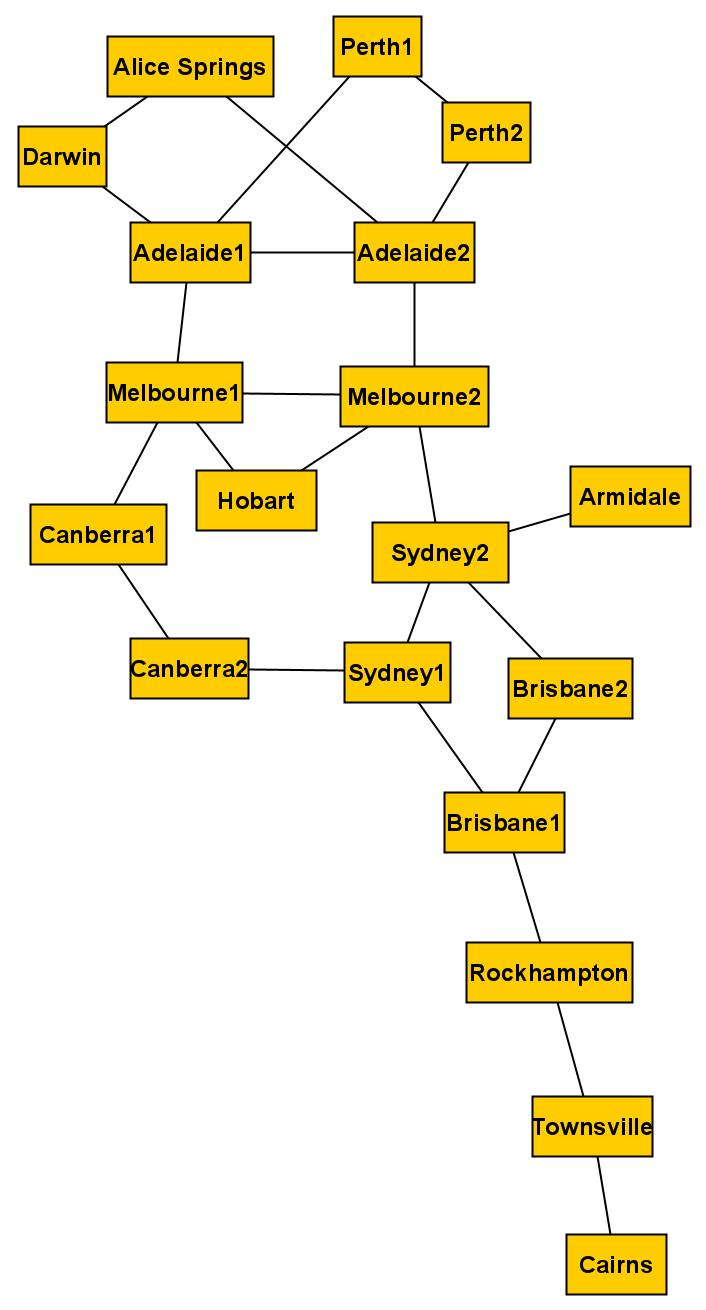
\includegraphics[width=0.65\linewidth]{Images/Aarnet_Graph.jpg}
	\caption{Original Aarnet Network (rearranged)}
	\label{fig:aarnet2009}
\end{figure}

\begin{figure}
	\centering
	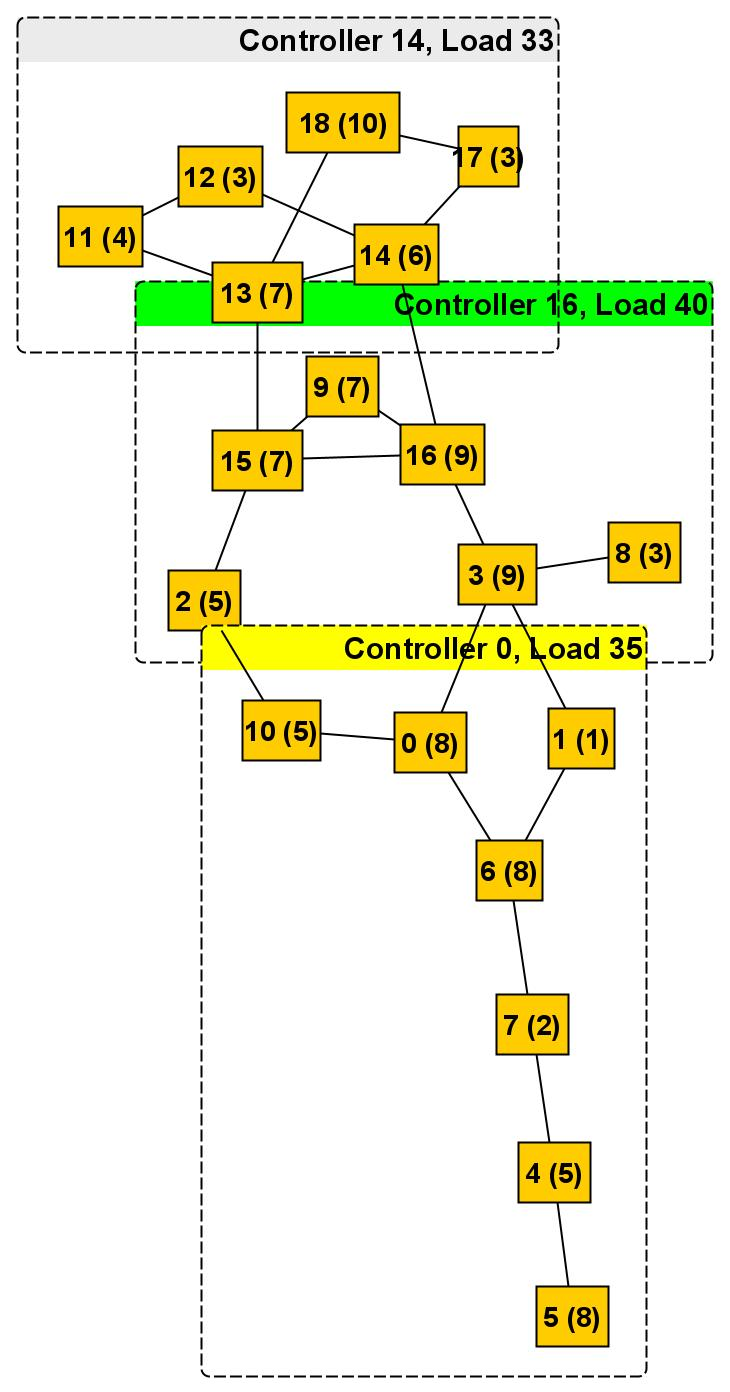
\includegraphics[width=0.65\linewidth]{Images/Aarnet_Load_1.jpg}
	\caption{Root state with no child state}
	\label{fig:aarnet2009l1}
\end{figure}

\begin{figure*}
	\centering
	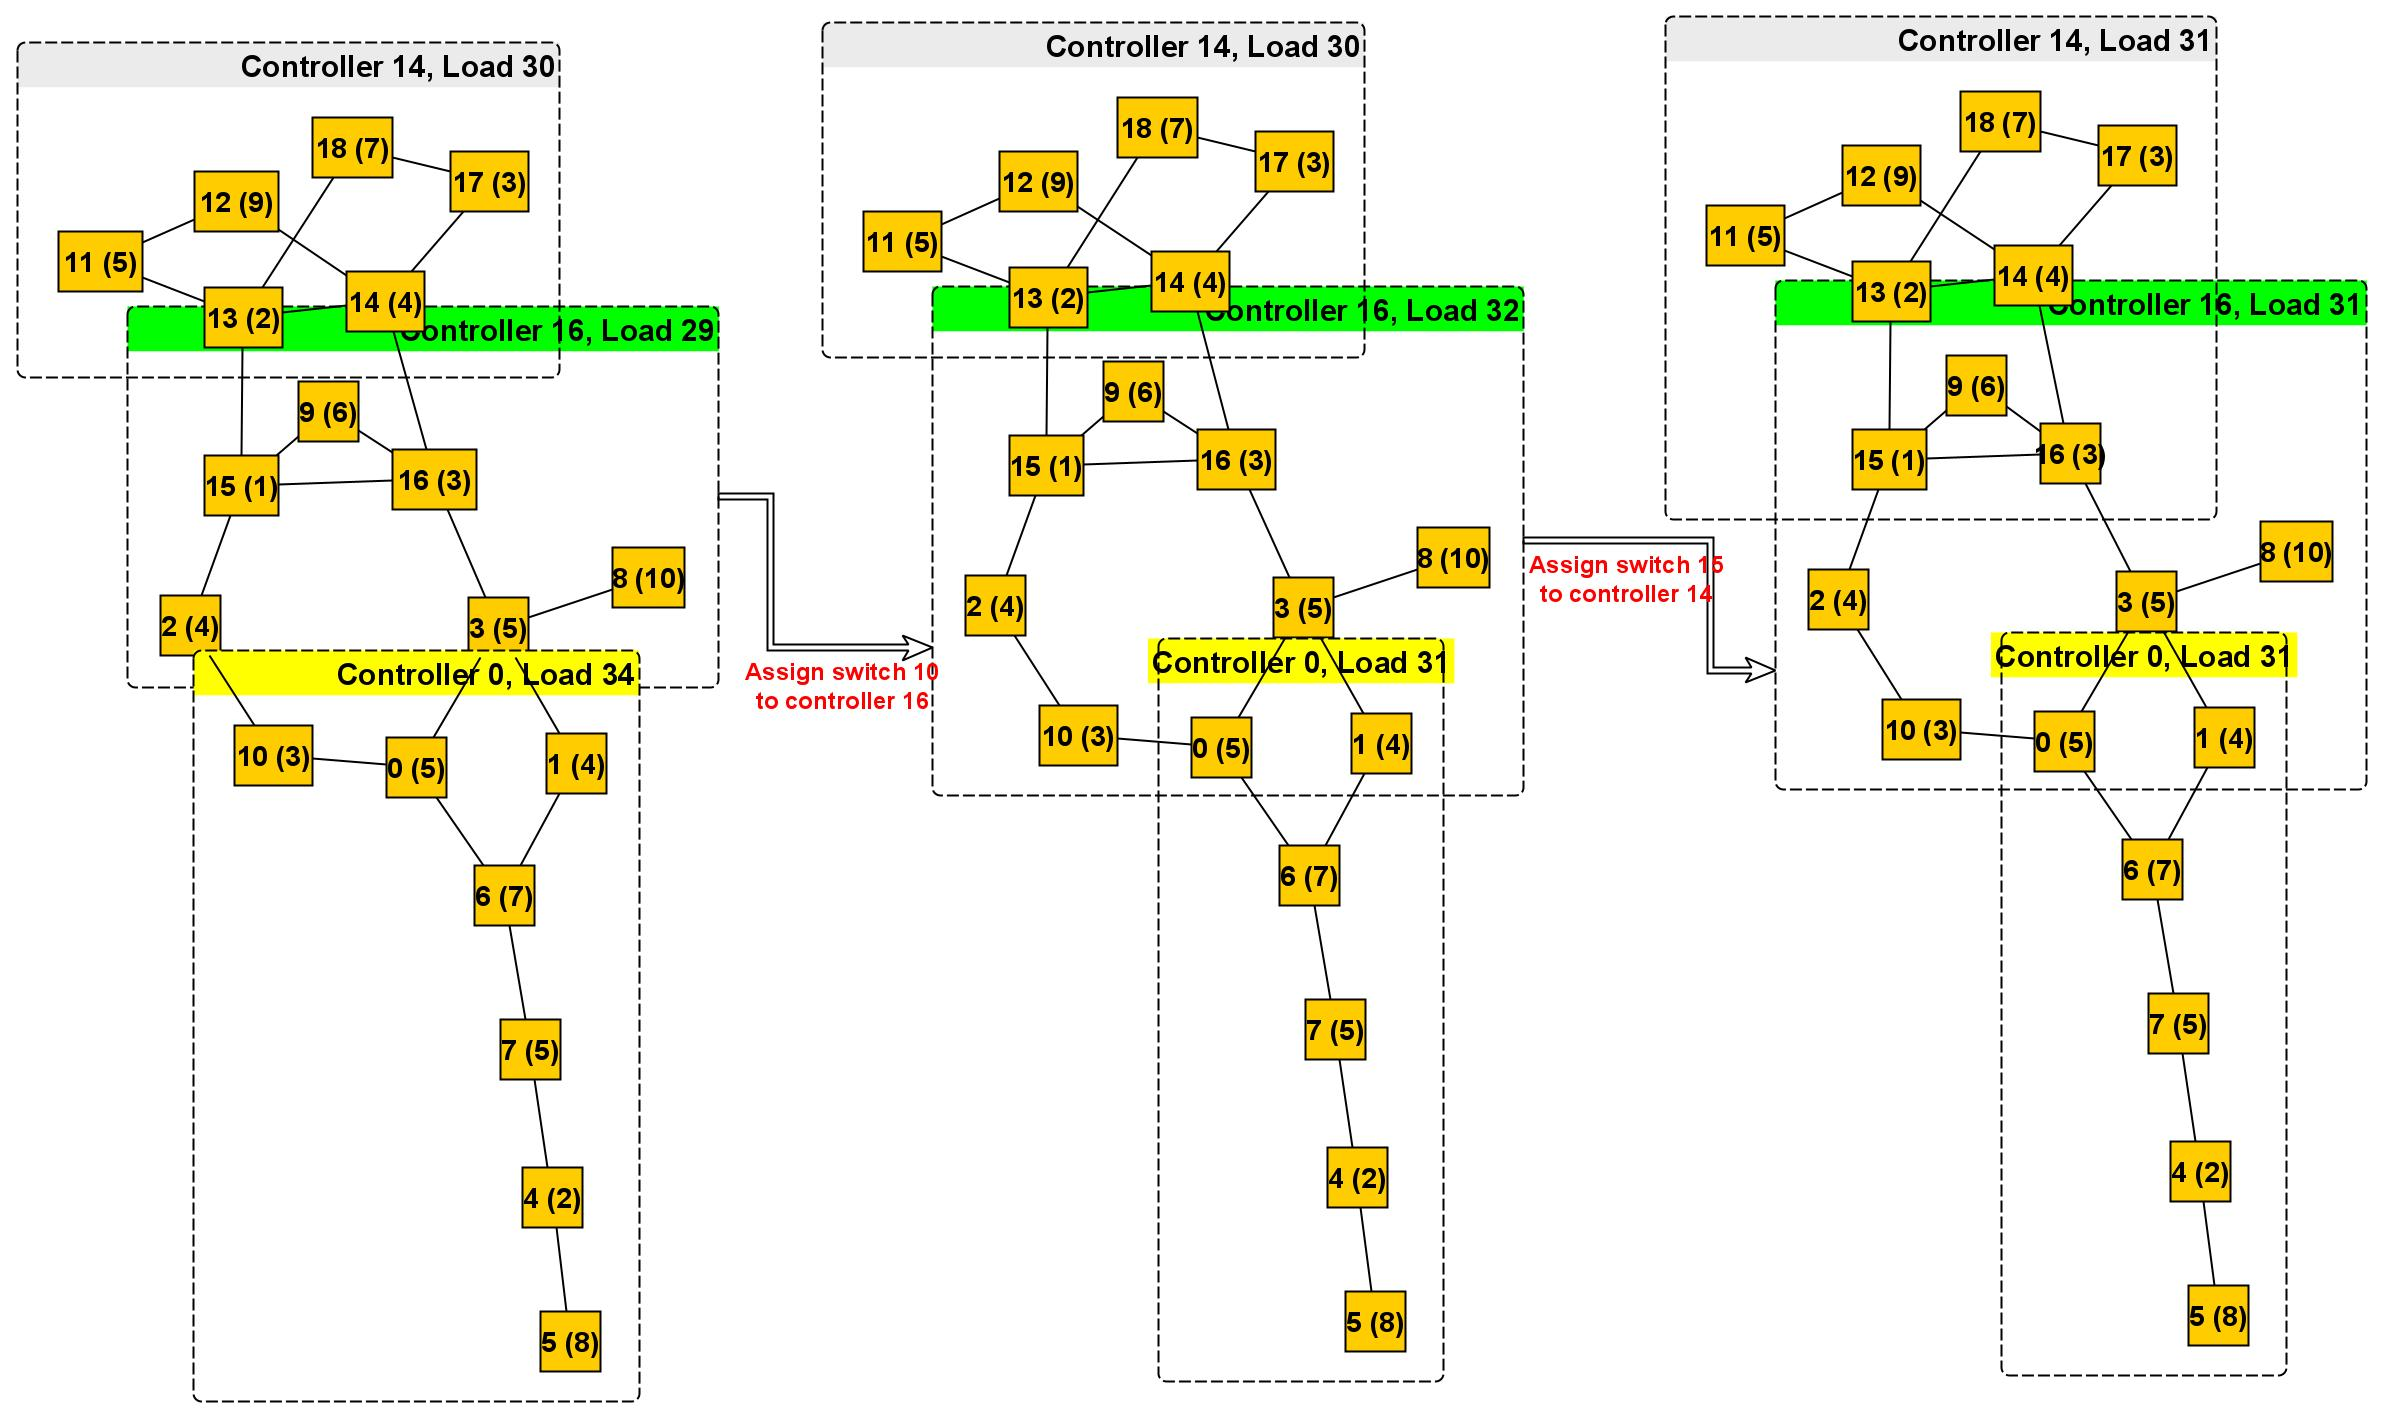
\includegraphics[width=\linewidth]{Images/Aarnet_Load_2.jpg}
	\caption{Optimal assignment scheme achieved after two iterations}
	\label{fig:aarnet2009l2}
\end{figure*}
%\caption{The GLBA algorithm applied on Aarnet Network variations with randomized loads, where each switch is represented by a switch id, followed by its load and each cluster has its own controller position and load marked above.}
%\label{fig:aarnet}

\noindent This section illustrates the application of GLBA on multiple load-balancing scenarios. The example topology used is an existing 19-node network of Australia, called \textit{Aarnet}. Figure \ref{fig:aarnet2009} shows the graph representation of the network and Figure \ref{fig:aarnet2009l1} is a state with no possible state generation (i.e., it is a leaf state). When GLBA is applied using a leaf state as root, the root state is returned - without any change. Contrarily, in Figure \ref{fig:aarnet2009l2}, the goal state is reached after two iterations. The initial load distribution is $30$ units for controller 14, $29$ units for controller 16, and $34$ units for controller 0. The total load is $93$ units, and the average load is $31$ unit. Table \ref{tab:example} represents the details of each iteration. The first column is the current iteration, the second column is the error of the current state, and the third column is the best heuristic value of all the generated states. In iteration 3, the algorithm will terminate and return the current assignment as the current heuristic is $0$.
	
\begin{table}
	\centering
	\caption{BLBA applied on example network (Fig. \ref{fig:aarnet2009l2})} \label{tab:example}
	\begin{tabular}{|l|c|c|}
		\hline
		\textbf{Iteration} & \textbf{Error} & \textbf{Best Heuristic} \\
		\hline
		1 & 14 & 2 \\
		\hline
		2 & 2 & 0 \\
		\hline
		3 & 0 & N/A \\
		\hline
	\end{tabular}
\end{table}

\section{Performance Analysis and Evaluation} \label{simulations}

\noindent The proposed mechanism clusters the network, places controllers, and performs load balancing on the clustered network after placement. The following sections \ref{SimEnv} and \ref{PerfMetrics} give a detailed description of the simulation environment and the performance metrics. In Section \ref{optimumK} optimum values for the decision variables, $k$ and $\alpha$ are determined.

\subsection{Simulation Environment} \label{SimEnv}
\noindent The simulation environment is developed using a high-level language C++, to perform experiments on existing network topologies collected from the Internet Topology Zoo \cite{knight2011internet}. The Topology Zoo contains a total of 261 existing networks, out of which a few ($18$) have islands (isolated nodes). Therefore, we perform our simulations on the remaining networks. A summary of the experimental networks is given in Table \ref{tab:zooSummary}.

\begin{table}
	\centering
	\caption{A summary of our Experimental Networks} \label{tab:zooSummary}
	\begin{tabular}{|l|c|}
		\hline
		\textbf{Category} & \textbf{Data} \\
		\hline
		Total number of networks & 243 \\
		\hline
		Number of unweighted networks & 134 \\
		\hline
		Maximum number of nodes & 754 \\
		\hline
		Minimum number of nodes & 4 \\
		\hline
		Networks with multi-edges & 82\\
		\hline
		Average Edge per Node & 1.285 \\
		\hline
	\end{tabular}
\end{table}

The initial weights of the links are their bandwidths in \textit{Gb/s} (Gigabits per second), which are converted into transmission latencies (milliseconds), assuming each control packet is 1500 bytes long. The maximum bandwidth is considered for links with variable bandwidths and all fiber-optic cables without available bandwidth information are assumed to have $1~Gb/s$ bandwidth. The networks with identical edge weights are considered as unweighted.

We perform our load balancing simulations on the network with the highest number of nodes ($|S|=754$) to illustrate the performance of GLBA. The switches are assumed to have loads of 1000 to 5000 in terms of active flows per second, which is equivalent to the loads of data-center switches \cite{benson2010traffic}. We assume the network has $10$ controllers that are placed using LBCA and LCSA, and each controller has a maximum processing capacity of $1000K~flows/s$ which is adequate to support the maximum load of the networks in our simulations.

\subsection{Performance Metrics} \label{PerfMetrics}

\begin{figure}
	\centering
	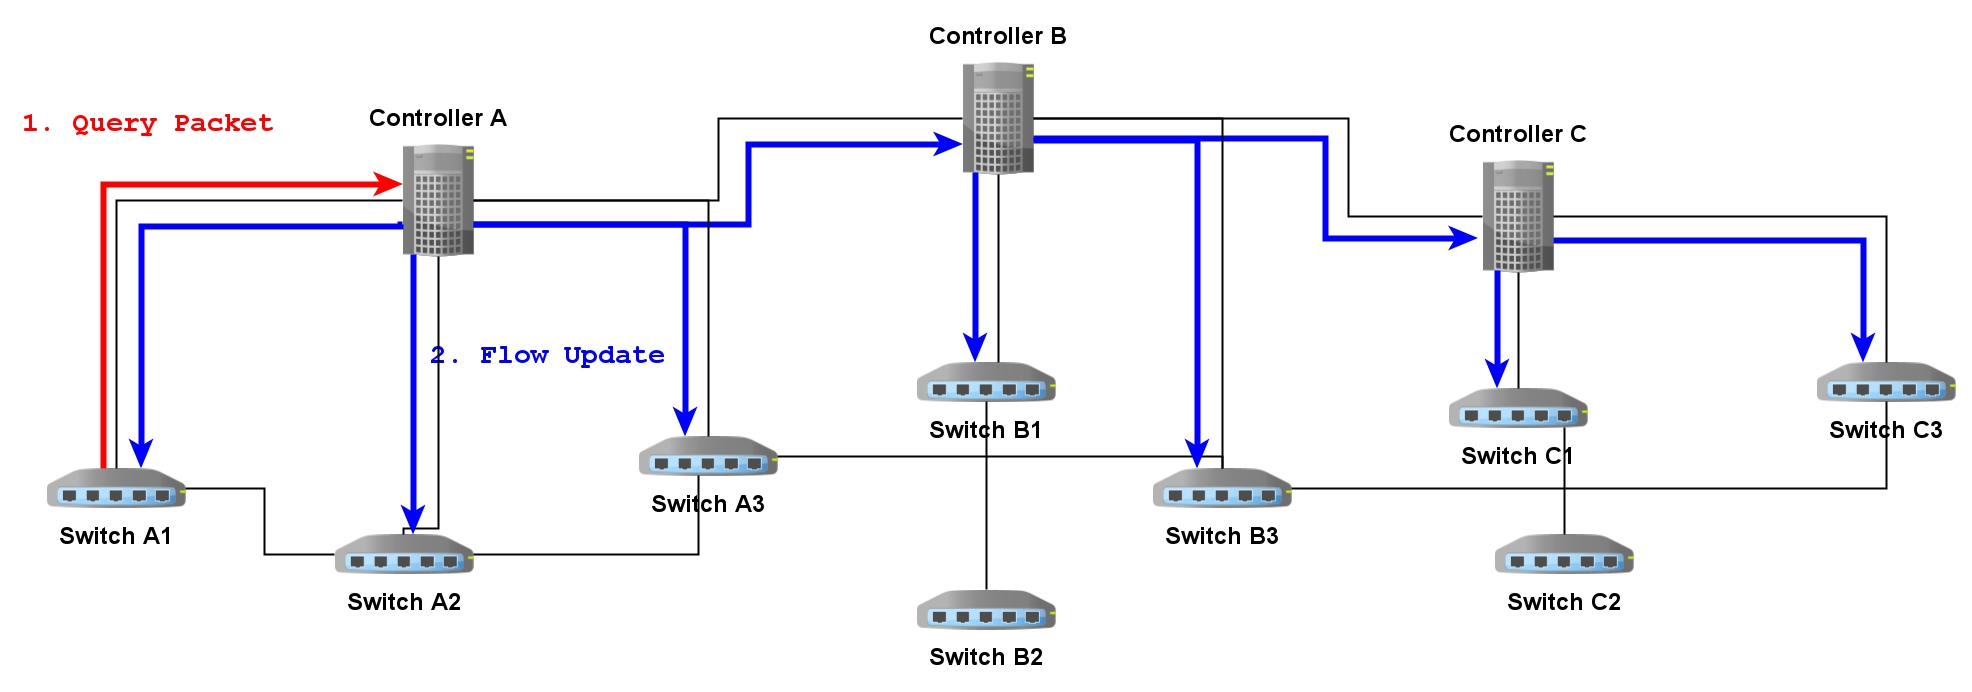
\includegraphics[width=0.95\linewidth]{Images/new_flow.jpg}
	\caption{Setup of a new flow in the flow tables of the switches in the network} \label{new_flow}
\end{figure}

\noindent SDN switches match every incoming packet with appropriate flow tables. The result of a match can either be a \textit{hit} - which means the appropriate flow is already in a flow table, or, a \textit{miss} - in which case the flow is new and the switch asks its assigned controller for the next course of action. The assigned controller calculates the path with the least delay for the flow and notifies the concerned switches to update their flow tables. However, for switches assigned to another controller, the corresponding controller is notified instead (Figure \ref{new_flow}). Therefore, the total time required to notify all the concerned switches about the new flow is the \textit{flow-setup latency}. We represent the average flow-setup latency ($\Omega_{avg}$) of the network as the average time to notify all possible pairs of switches in the network. For a network with $|S|$ switches, the average flow-setup latency can be calculated as follows:

\begin{equation} \label{eqn:setupLatency}
\Omega_{avg} = \frac{\sum_{s_i,s_d\in S} \left(dis(s_i,c_i)+ maxPath(s_i,s_d)\right)}{|S|\times |S-1|}
\end{equation}

\begin{equation}
maxPath(s_i,s_d) = \max_{x\in path(i,d)}\left(dis(c_i,c_x)+dis(c_x,s_x) \right)
\end{equation}

where, $path(i,d)$ is the path with least delay from source $s_i$ to destination $s_d$, and $s_x$ is any switch in that path. The controllers of switches $s_i$ and $s_x$ are $c_i$ and $c_x$ respectively.

The system time (service + waiting time) of the controllers increase significantly for an imbalanced network, which can be calculated if the loads of the switches and controllers are known. Accordingly, the overall flow setup latency for a network $S$ is the maximum time any switch needs to install a new-flow rule, and is denoted by:
\begin{equation}
\Omega_S = \max_{s_i\in S} \bigg( \Delta_{s_i}\times l_{s_i} \bigg)
\end{equation}

where $\Delta_{s_i}$ is the average time required for a switch $s_i$ to add a new flow to its flow table and $l_{s_i}$ is the switch load. Using the average flow-setup latency (Equation \ref{eqn:setupLatency}) and average controller response times (Equation \ref{eqn:cresponse}) of a network, $\Delta_{s_i}$ is derived as follows:
\begin{equation}
\Delta_{s_i} = \frac{\sum_{s_i,s_d\in S} \bigg[dis(s_i,c_i)+RT_{c_i}+maxPath(s_i,s_d) \bigg]}{|S|-1}
\end{equation}

\begin{equation}
maxPath(s_i,s_d) = \max_{s_j\in path_{id}}\{dis(c_i,c_j)+RT_{c_j}+dis(c_j,s_j)\}
\end{equation}

where $RT_{c_i}$  and $RT_{c_j}$ are the average controller response times for controllers $c_i$ and $c_j$ respectively.

\subsection{Decisive Variables} \label{optimumK}

\begin{figure}[t]
	\centering
	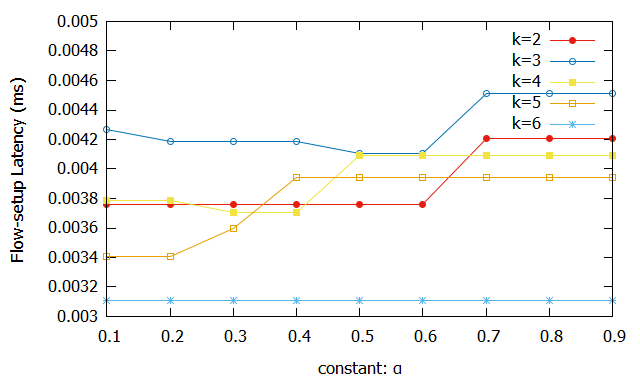
\includegraphics[width=0.95\linewidth]{Images/Abilene_Analysis.png}
	\caption{Average flow-setup latencies for varying values of $\alpha$ and $k$ in a network containing $|S|=11$ switches} \label{fig:abileneA}
\end{figure}

\noindent LBCA clusters the network into $k$ sub-networks and LCSA places a controller in each sub-network using the constant $\alpha$, which is a real number ranging from $0$ to $1$. The constant dictates the placement of controllers by controlling the priority of intra-cluster and inter-cluster distances. Applying LBCA on a small network with varying values of $k$ and $\alpha$ (Figure \ref{fig:abileneA}) provides valuable insight on how the two variables affect the overall flow-setup latency of a network (Equation \ref{eqn:setupLatency}).

An increased number of clusters are formed when an excessively large amount of controllers are placed in a network. Consequently, the cluster-sizes are diminished, greatly reducing the number of viable controller positions in a specific cluster. Therefore, for a specific and large value of $k$, varying the value of $\alpha$ causes little or no change in placement and has no effect on overall flow-setup latency ($k=6$). For smaller values of $k$, the flow-setup latency gradually decreases and then increases ($k<5$). In some cases, the latency only increases as inter-controller distances increase ($k=5$), which indicates that no better placement is found for greater controller separation. The flow-setup latency is the lowest when $\alpha \ge 0.2$ and $\alpha \le 0.6$, which indicates that inter-controller communication contributes more to the flow-setup procedure when there are many controllers. However, in our experiments, we have used $\alpha=0.5$ to give equal priority to controller-to-switch and controller-to-controller communication.

\begin{figure}
	\centering
	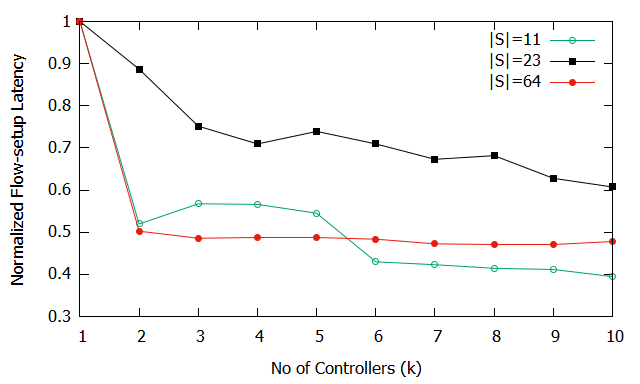
\includegraphics[width=0.95\linewidth]{Images/k_vs_l.png}
	\caption{Decreasing average flow-setup latencies with respect to number of controllers ($k$) for different networks. As the networks have varying latencies, they are normalized for comparison.} \label{fig:KvsL}
\end{figure}

The flow-setup latency of a network decreases as the number of controllers increase, with a few exceptions due to variations in network topology (Figure \ref{fig:KvsL}). The rate of decrease is greater for smaller networks compared to larger networks as controller/switch ratio increase drastically for smaller networks. Accordingly, the setup latency is minimum when $k$ is equal to the total number of nodes in a network, which, however, invalidates one of the firsthand benefits of placing controllers (simplifying nodes and reducing costs). In order to determine the optimum number of controller $k$ for a network $S$, we define an improvement ratio:

\begin{equation}
Improvement~Ratio_k = \frac{Latency_1}{Latency_k\times k}
\end{equation}

where $Latency_1$ and $Latency_k$ are the flow-setup latencies when the number of controllers is 1 and $k$ respectively.

\begin{figure}[t]
	\centering
	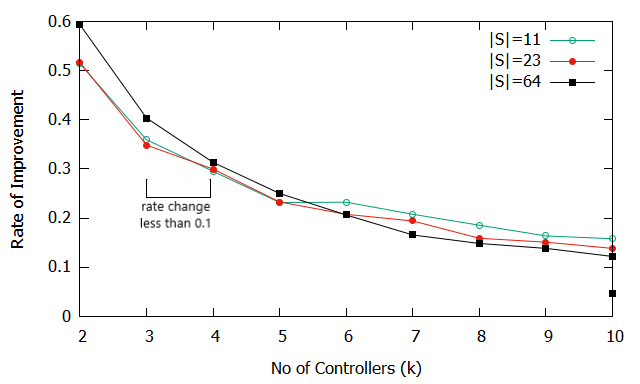
\includegraphics[width=0.95\linewidth]{Images/cutoff.png}
	\caption{Gradually decreasing improvement ratio with respect to number of controllers ($k$) for networks of different sizes} \label{fig:cutoff}
\end{figure}

The improvement ratio for a network decreases gradually with respect to increasing number of controllers (Figure \ref{fig:cutoff}). We observe that the improvement rate \textit{change} decreases drastically to less than $0.1$ from more than $0.2$ and $0.15$, after adding 4 controllers to the network where $|S|=64$ and 3 controllers to the other two networks, respectively. Therefore, we cease adding controllers when the improvement rate change drops below $0.1$. Consequently, the resultant average switch/controller ratio of the 238 networks is $12.79$. According to expert opinions \cite{heller2012latency}, a network with $34$ nodes requires approximately $3$ controllers to function efficiently and one more to handle failures, which supports our optimal $k$ derivation in terms of average switch/controller ratio.

\section{Simulation Results} \label{simulationResults}
In the following sections \ref{CPAnalysis} and \ref{LoadAnalysis}, our proposed algorithms are validated by comparing them with the state-of-the-art controller placement \cite{dbcp2017} and load balancing algorithms \cite{filali2018sdn}, respectively.

\subsection{Controller Placement} \label{CPAnalysis}

\noindent In this section, we evaluate our static controller placement method (LBCA+LCSA) by comparing it to the well-known algorithm DBCP \cite{dbcp2017} and the algorithm DBC \cite{aziz2019degree}. DBCP places controllers based on the density of nodes and the minimum distance to higher density nodes. In order to compare the algorithms, we simulate both DBC and LBCA with the same number of controllers as DBCP when clustering the networks from the Zoo Topology. DBCP underperforms compared to LBCA and DBC when the network has high connectivity (e.g. star topology) or when all nodes have an equal density (e.g. ring topology). Our simulations using the remaining networks suggest that LBCA+LCSA outperforms both DBCP and DBC in terms of flow-setup latencies.

\begin{figure}
	\centering
	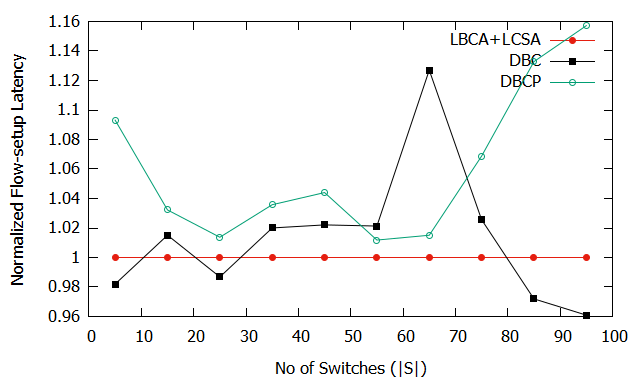
\includegraphics[width=\linewidth]{Images/edited_forced_comparison.png}
	\caption{Comparison among LBCA+LCSA, DBCP and DBC, in terms of normalized flow-setup latency} \label{fig:Fcomparison}
\end{figure}

The flow-setup latency results of the simulations vary greatly for different networks. Therefore, we represent the latencies of DBCP and DBC as a ratio of the latencies of LBCA+LCSA and plot their averages for a given range of network sizes (Figure \ref{fig:Fcomparison}). The average latency of all the networks with network sizes less than $10$ are plotted for $|S|=5$, those greater than 9 and less than 20 are plotted for $|S|=15$, and so on. Although DBC performs better for certain unweighted networks, LBCA+LCSA outperforms both DBCP and DBC in 78\% and 72\% of the simulated networks, respectively.

\subsection{Load Balancing} \label{LoadAnalysis}

\begin{figure}
	\centering
	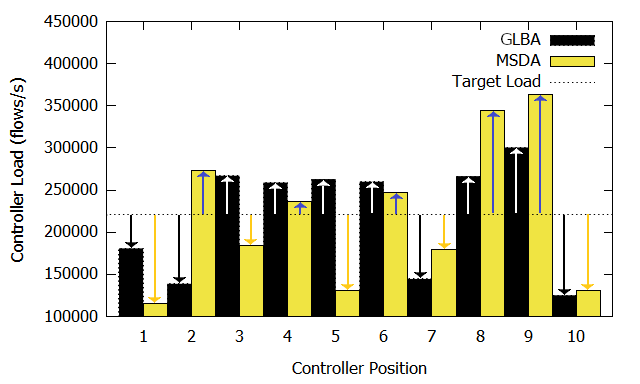
\includegraphics[width=\linewidth]{Images/load_comparison_edit.png}
	\caption{Comparison between GLBA and MSDA in terms of load per controller} \label{fig:Lcomparison}
\end{figure}

\noindent GLBA balances the loads of the controllers by swapping clusters of border nodes to avoid overlapping cluster formations. We set the maximum iteration limit of GLBA to $100$ and compare with the algorithm MSDA \cite{filali2018sdn, fragiadakis2016matching} in terms of maximum load imbalance. The loads of the switches are randomly assigned within the range of $1000$ to $5000$ with equal probability. Therefore, the average switch load is $2500 flows/s$ and the target controller load is $188.5K flows/s$ (Figure \ref{fig:Lcomparison}). The global precedence list of MSDA is calculated by multiplying transmission latency with average sojourn time or controller processing time. However, in our experiments, we observe that transmission latencies are greater than processing latencies, which results in load imbalance. Furthermore, when the maximum controller capacity is decreased substantially, MSDA underperforms as the preferences of the controllers and switches cannot be satisfied. The simulation suggests that GLBA outperforms MSDA in terms of controller load, especially for controllers 8 and 9 (Figure \ref{fig:Lcomparison}). Although the algorithm converges after 10 iterations approximately, the maximum iteration limit can be increased for better accuracy and performance.

\begin{figure}
	\centering
	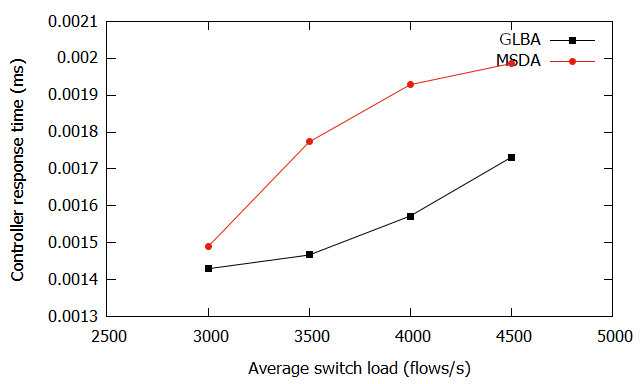
\includegraphics[width=\linewidth]{Images/response_comparison_edit.png}
	\caption{Gradually decreasing average response times for varying switch loads} \label{fig:Rcomparison}
\end{figure}

Figure \ref{fig:Rcomparison} represents the comparison between GLBA and MSDA in terms of maximum controller response times for different average switch loads. The response times increase with increasing switch loads as the controller loads also increase significantly. The comparison shows that GLBA outperforms MSDA in terms of average controller response times. The average controller response time is reduced by an average of $13\%$.

\begin{figure}
	\centering
	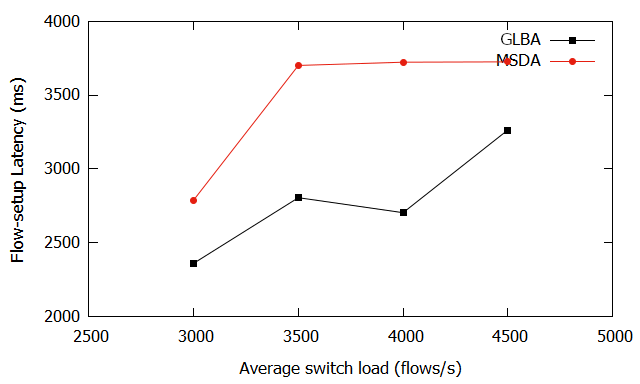
\includegraphics[width=\linewidth]{Images/omega_comparison_edit.png}
	\caption{Comparison between GLBA and MSDA in terms of maximum flow-setup latency} \label{fig:Ocomparison}
\end{figure}

We also compare both the algorithms in terms of maximum flow setup latency of a switch in Figure \ref{fig:Ocomparison} and observe that GLBA outperforms MSDA. The flow-setup latency for higher average switch loads shows the minimum change for MSDA as the controller-switch preferences are prioritized. GLBA on the other hand reduces latency as long as a local optimum is available. Consequently, the algorithm terminates when further optimization causes overlapping clusters (producing unnecessary traffic), which is observed for an average switch load of 3500 flows/s.

\section{Conclusion} \label{conclusion}

\noindent In this paper, we propose a novel controller assignment mechanism that clusters the network, places controllers, and balances loads to reduce the overall flow-setup latency of the network. Our proposed method addresses the Controller Placement Problem (CPP) and outperforms multiple state-of-the-art algorithms based on various performance metrics. Our proposed method has many advantages over other algorithms which include - having polynomial time complexity, providing an optimal number of clusters, decreasing controller response time, and flow-setup latency simultaneously. Our proposed algorithm GLBA can be extended to optimize any parameter by introducing and improving different error functions. Future work can include variable controller capacities when balancing controller loads. Our proposed method can also be extended to facilitate simultaneous optimization of several core network parameters, which will be significantly helpful for network operators.

%% Loading bibliography style file
%\bibliographystyle{model1-num-names}
\bibliographystyle{cas-model2-names}

% Loading bibliography database
\bibliography{mybib}

\end{document}

